% see handdrawn figure on paper

\documentclass{standalone}
\usepackage[dvipsnames]{xcolor}
\usepackage{tikz,amsmath,amssymb}
\usepackage{tikz-3dplot}
\usetikzlibrary{shapes,calc,positioning,arrows,intersections}

\begin{document}
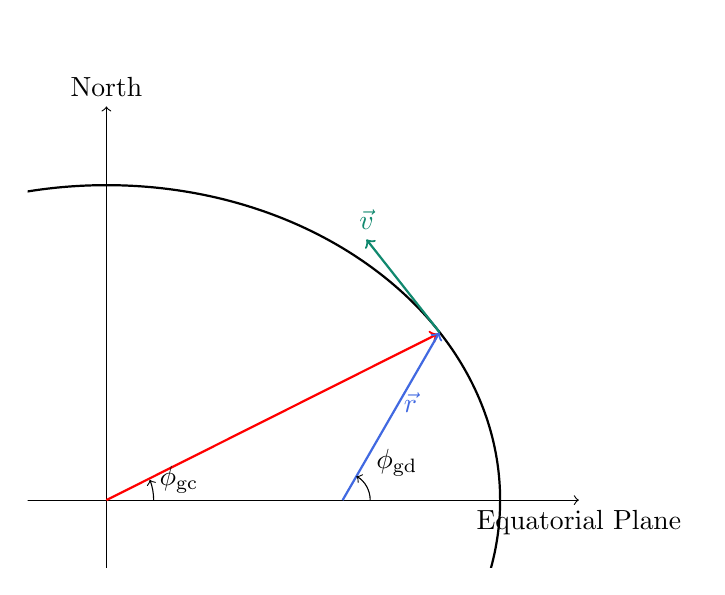
\begin{tikzpicture}
\clip (-1,-0.85) rectangle (7.5,6.);
% Define the orbit
\pgfmathsetmacro{\t}{60} % True Anomaly value, deg
\pgfmathsetmacro{\e}{0.6} % Eccentricity
\pgfmathsetmacro{\a}{5} % Semi-Major Axis, cm
\pgfmathsetmacro{\v}{1.5} % Bogus velocity vector size, cm
 
% Compute some useful quantities
\pgfmathsetmacro{\b}{\a*sqrt(1-\e^2)} % Semi-Minor Axis, cm
\pgfmathsetmacro{\p}{\a*(1-\e^2)} % Semi-Latus Rectum, cm
\pgfmathsetmacro{\r}{ \p / (1 + \e*cos(\t))} % Radius, cm
\pgfmathsetmacro{\g}{atan(\r*\e*sin(\t) / \p)} % Flight path angle, deg
\pgfmathsetmacro{\eccanom}{atan(1-\e^2)*sin(\t) /  (1 + \e*cos(\t)))} % eccentric anomaly, deg
 
% Orbit reference frame, orbit, attracting body
\draw[->]({-\a-1},0) -- ({\a+1},0) node[anchor=north] {Equatorial Plane};
\draw[->](0, {-\b-1}) -- (0,{\b + 1}) node[anchor=south] {North};
\draw[thick] (0,0) ellipse ({\a} and {\b});
 
% h-direction
%\draw[->] (0.25,0) arc (0:340:0.25) node[anchor=north west] {$\hat{h}$};
 
% Move center to attractive focus to make plotting easier
\begin{scope}[shift={({\a*\e},0)}]
 
% Position and Velocity vectors
\draw[thick,Red, ->]({-\a*\e},0) -- ({0.98*\r*cos(\t)}, {0.99*\r*sin(\t)});
%\draw ( {0.35*cos(\t/2)}, {0.35*sin(\t/2)} ) node[anchor=south west] {$\phi_\text{gc}$};

\draw[->]({-\a*\e +0.6},0) arc (0:\eccanom:0.7) node[anchor=west]  {$\phi_\text{gc}$};

\draw[thick,RoyalBlue, ->](0,0) -- ({\r*cos(\t)}, {\r*sin(\t)});
\draw[RoyalBlue] ({0.7*\r*cos(\t)}, {0.7*\r*sin(\t)}) node[anchor=north ]{$\vec{r}$};
\draw[thick,PineGreen, ->]({\r*cos(\t)}, {\r*sin(\t)}) -- ({\r*cos(\t) + \v*cos(\t + 90 -\g)}, {\r*sin(\t) + \v*sin(\t + 90 -\g)}) node[anchor=south]{$\vec{v}$};
 
%\filldraw({\r*cos(\t)}, {\r*sin(\t)}) circle (0.05);
 
% Orbit frame Coordinates
%\draw[RoyalBlue, ->] ({\r*cos(\t)}, {\r*sin(\t)}) -- ({(\r+1)*cos(\t)}, {(\r+1)*sin(\t)}) node[anchor=south]{$\hat{r}$};
%\draw[Blue, ->] ({\r*cos(\t)}, {\r*sin(\t)}) -- ($ ({\r*cos(\t)}, {\r*sin(\t)}) + ({-sin(\t)}, {cos(\t)}) $) node[anchor=north] {$\hat{\theta}$};
% 
% True Anomaly
\draw[->](0.35,0) arc (0:\t:0.35);
\draw ( {0.35*cos(\t/2)}, {0.35*sin(\t/2)} ) node[anchor=south west] {$\phi_\text{gd}$};
 
% Flightpath Angle
%\draw[->] ($ ({\r*cos(\t)}, {\r*sin(\t)}) + ({-0.35*sin(\t)}, {0.35*cos(\t)}) $) arc ({\t+90}:{\t+90-\g}:0.35) node[anchor=north east] {$\gamma$};
% 
% Attractive Focus - Last to cover up radial vector
%\filldraw (0,0) circle (0.25);
\end{scope}
 
\end{tikzpicture}
\end{document}
